\documentclass[tikz,crop]{standalone}

\usetikzlibrary{
  positioning,
  arrows,
  fit,
  decorations.pathreplacing,
  backgrounds
}

\begin{document}
  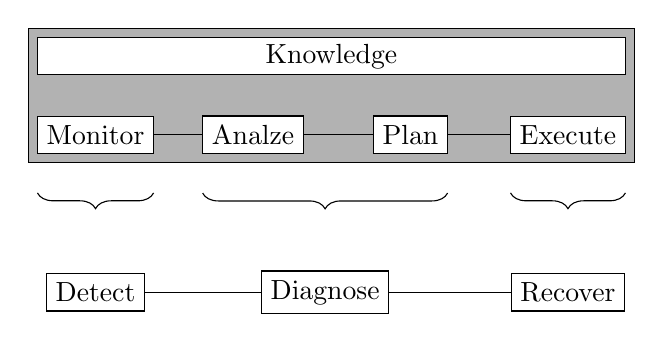
\begin{tikzpicture}[
    auto,node distance=2cm,
    stepNode/.style={draw,fill=white,outer sep=0pt},
    correspondence/.style={decorate,decoration={brace,amplitude=.2cm,mirror,raise=.5cm}}
  ]
    % MAPE-K loop
    \node[stepNode] (monitor) {Monitor};
    \node[stepNode, right of=monitor] (analyze) {Analze};
    \node[stepNode, right of=analyze] (plan) {Plan};
    \node[stepNode, right of=plan] (execute) {Execute};
    \node[stepNode,inner sep=0pt,fit={(monitor) (execute)},yshift=1cm,label=center:Knowledge] (knowledge) {};
    
    \begin{scope}[on background layer]
      \node[draw,fill=black!30,fit={(knowledge) (monitor) (analyze) (plan) (execute)}] (mapek) {};
    \end{scope}
    
    \draw[-,black] (monitor) -- (analyze)  -- (plan) -- (execute);
    
    % self-healing loop
    \node[stepNode, below of=monitor] (detect) {Detect};
    \node[fit={(analyze) (plan)}] (diagnose anchor) {};
    \node[stepNode, below of=diagnose anchor] (diagnose) {Diagnose};
    \node[stepNode, below of=execute] (recover) {Recover};
    
    \draw[-,black] (detect) -- (diagnose) -- (recover);
    
    % correspondences
    \draw[correspondence] (monitor.south west) -- (monitor.south east);
    \draw[correspondence] (analyze.south west) -- (plan.south east);
    \draw[correspondence] (execute.south west) -- (execute.south east);
  \end{tikzpicture}
\end{document}